\documentclass[portuguese,11pt,a4paper,titlepage]{article}

\usepackage{graphicx}
\usepackage{fancyhdr}
\usepackage[portuguese]{babel}
\usepackage{blindtext}
\usepackage{color}
\usepackage{listings}
\usepackage[T1]{fontenc}
\usepackage[margin=3cm]{geometry}
\usepackage[final]{pdfpages}
\usepackage{siunitx}
\usepackage[framed, numbered]{matlab-prettifier}
\usepackage{wrapfig}
\usepackage{subcaption}
\usepackage{hyperref}

\hypersetup{
    colorlinks,
    citecolor=black,
    filecolor=black,
    linkcolor=black,
    urlcolor=black
}

\newcommand{\nextyear}{\advance\year by 1 \the\year\advance\year by -1}

\setlength{\headheight}{14.2pt}
\fancypagestyle{fancy}{
	\fancyhf{}
	\fancyhead[C]{A01 - speed\_run}
	\fancyfoot[R]{
		\textsf{\thepage}
	}
	\fancyfoot[L]{
		\textsf{AED - \the\year/\nextyear}
	}
	\fancyfoot[C]{
\includegraphics[height=.7cm]{ua.pdf}}
	\renewcommand{\headrulewidth}{0pt}
}
\pagestyle{fancy}

\definecolor{mygreen}{rgb}{0,0.6,0}
\definecolor{mygray}{rgb}{0.5,0.5,0.5}
\definecolor{mymauve}{rgb}{0.58,0,0.82}

\lstdefinestyle{c_without_comments}
{
	  style=c_with_comments,
	    morecomment  = [l][\@gobble]{//},
		  morecomment  = [is]{/*}{*/},
}
\lstset{ 
	backgroundcolor=\color{white},   % choose the background color; you must add \usepackage{color} or \usepackage{xcolor}; should come as last argument
	basicstyle=\small\ttfamily,      % the size of the fonts that are used for the code
	breakatwhitespace=false,         % sets if automatic breaks should only happen at whitespace
	breaklines=true,                 % sets automatic line breaking
	captionpos=b,                    % sets the caption-position to bottom
	commentstyle=\color{mygreen},    % comment style
	extendedchars=true,              % lets you use non-ASCII characters; for 8-bits encodings only, does not work with UTF-8
	frameround=tttt,
	frame=single,	                 % adds a frame around the code
	keepspaces=true,                 % keeps spaces in text, useful for keeping indentation of code (possibly needs columns=flexible)
	keywordstyle=\color{blue},       % keyword style
	language=C,                      % the language of the code
	morekeywords={*,\ldots},         % if you want to add more keywords to the set
	numbers=left,                    % where to put the line-numbers; possible values are (none, left, right)
	numbers=none,
	rulecolor=\color{black},         % if not set, the frame-color may be changed on line-breaks within not-black text (e.g. comments (green here))
	showspaces=false,                % show spaces everywhere adding particular underscores; it overrides 'showstringspaces'
	showstringspaces=false,          % underline spaces within strings only
	showtabs=false,                  % show tabs within strings adding particular underscores
	stringstyle=\color{mymauve},     % string literal style
	tabsize=2,                       % sets default tabsize to 2 spaces
}


\newcommand{\foreign}[1]{\textit{#1}}
\newcommand{\srcdir}{..}
\newcommand{\matlabdir}{"../MATLAB-fittings"}

\title{ \normalsize Licenciatura em Engenharia Informática\vskip 1.5em
		\Huge Algoritmos e Estruturas de Dados\vskip .7em
		\bfseries speed\_run\vskip 1.5em
		
\includegraphics{ua.pdf}
}
\author{
	João Catarino\\NMec: 93096\\\%\and Rúben Garrido\\NMec: 107927\\\%\and Nuno Vieira\\NMec: 107283\\\%
}
\date{\today}

\begin{document}
\maketitle

\tableofcontents
\pagebreak

\section{Introdução}
Este trabalho consiste em desenvolver algoritmos capazes de resolver o seguinte problema:

Uma estrada encontra-se dividida em vários segmentos de igual tamanho, cada um com uma velocidade pré-definida.
O objetivo deste problema é encontrar o menor número de passos necessários para percorrer a estrada, começando no primeiro segmento e terminando no último, com velocidade 1.

Em cada passo, é possível avançar para os segmentos seguintes, com velocidade igual à velocidade de chegada ao segmento atual
ou inferior/superior à velocidade atual em 1 unidade.
Contudo, em cada iteração, deve-se verificar se a velocidade de partida é igual ou inferior à velocidade dos segmentos seguintes.
Caso a velocidade atual seja 1, não é possível reduzir a velocidade.

\section{Soluções}
A solução original utiliza uma função recursiva para verificar todas as combinações
de passos a todas as velocidades possíveis dentro dos limites de cada casa,
guardando sempre a melhor solução encontrada até ao momento. Esta possui um tempo
de execução com ordem de grandeza \begin{math}10^{154}\end{math} (em anos) para a resolução do caso \begin{math}n = 800\end{math}.
Com vista a obter a solução em tempo aceitável, foram criadas três soluções capazes de
o fazer na ordem dos microsegundos. A primeira altera apenas ligeiramente a
solução original, enquanto que a segunda é não recursiva (dinâmica) e utiliza o princípio da solução anterior
com algumas optimizações. A terceira combina as duas soluções anteriores.
\subsection{Original}
A solução dada é recursiva e itera sobre todas as possibilidades de
percurso, guardando a melhor solução até ao momento.

Esta parte das soluções de maior número de passos (menor velocidade por passo) para
as de menor número de passos (maior velocidade por passo) dentro das regras do problema.

Pelo facto de a solução ser recursiva, à medida que o tamanho do problema aumenta,
o número de chamadas recursivas também aumenta, o que leva a um tempo de execução exponencial.
Por exemplo, a partir de \begin{math}n = 35\end{math}, o tempo de execução é superior a 1 segundo,
pelo que esta não é, portanto, uma solução viável para o problema. 

\subsection{Original Improved} \label{original_improved}
A presente solução introduz duas pequenas mudanças no código original, que, no entanto,
geram alterações significativas no seu comportamento.

Em primeiro lugar, é introduzido controlo de fluxo através de um valor de retorno
\foreign{boolean} (implementado como inteiro).
\lstinputlisting[linerange={167-169}]{\srcdir/speed\_run.c}
Se uma sequência de chamadas recursivas chegar a uma solução, a última chamada
retorna 1. \lstinputlisting[linerange={166-167}]{\srcdir/speed\_run.c}
Neste caso, as chamadas anteriores retornarão também 1.
Isto significa que o programa grava apenas a primeira solução que encontrar.
\lstinputlisting[linerange={153-158}]{\srcdir/speed\_run.c}
Deste modo, torna-se imperativo que o programa encontre a melhor solução possível
à primeira tentativa. Esta condição implica que o ``carro'' se mova o mais rápido possível
em qualquer passo para obter o menor número de passos. A segunda alteração
garante essa condição, ao fazer com que o programa itere
desde as maiores velocidades para as menores.
\lstinputlisting[linerange={163-164}]{\srcdir/speed\_run.c}

\subsection{Advance and retreat}
O algoritmo Advance and retreat foi feito de raiz. O seu princípio 
consiste em tentar, a qualquer passo, avançar com a velocidade mais alta.
Em cada passo, a escolha de velocidade é representada por um incremento
($-$1, 0 ou 1). O programa começa sempre por tentar o maior incremento.
Para verificar passos possíveis, utilizam-se os seguintes métodos:

Calcular a distância de paragem para cada velocidade possível em cada passo para evitar correr para além do fim do
trajeto:
\lstinputlisting[firstline=125, lastline=135]{\srcdir/speed\_run.c}

Verificar, a partir do incremento mais alto, se uma ``passada'' não  quebra
os limites de velocidade das casas pelas quais passaria:
\lstinputlisting[firstline=196, lastline=203]{\srcdir/speed\_run.c}

Realizado o passo, a escolha do incremento é guardada num \foreign{array},
na posição associada ao número do passo. Desta forma, este \foreign{array}
guarda as escolhas feitas até ao passo atual.
\lstinputlisting[firstline=217, lastline=231]{\srcdir/speed\_run.c}
Quando um passo é impossível de executar a qualquer das velocidades possíveis,
o algoritmo recua um passo e tenta reduzir o incremento de velocidade até que
consiga avançar novamente. Não sendo possível avançar com nenhum dos incrementos,
o programa recua novamente, e assim sucessivamente.
\lstinputlisting[firstline=263, lastline=265]{\srcdir/speed\_run.c}
\subsection{Combined}
Com esta solução, tentou-se aproximar o comportamento do algoritmo
\foreign{Original Improved} à solução \foreign{Advance and Retreat}, com o
objetivo de observar diferenças entre uma solução dinâmica e recursiva com
lógica semelhante.
Para tal, ao invés de, no ciclo \verb#for#, existir uma verificação de
\foreign{overstep} para passo, utilizou-se a função \verb#valstop#, presente no algoritmo \foreign{Advance and retreat}.
\lstinputlisting[firstline=307, lastline=316]{\srcdir/speed\_run.c}
\pagebreak

\section{PDFs de soluções}
\subsection{Original Improved}
\includegraphics[width=\textwidth]{800_2.pdf}
\subsection{Advance and retreat}
\includegraphics[width=\textwidth]{800_3.pdf}
\subsection{Combined}
\includegraphics[width=\textwidth]{800_4.pdf}
\pagebreak

\section{Tempos de execução e estimativas}
\subsection{Original}
Devido à complexidade do algoritmo, não foi possível obter tempos de execução para \begin{math}n = 800\end{math},
pelo que foi necessário recorrer a estimativas, utilizando o MATLAB.

Procedeu-se ao ajuste de uma curva do tipo \begin{math}a\times e^{bx}\end{math}
aos tempos obtidos até uma hora, utilizando a Curve Fitting Toolbox do MATLAB.
De seguida, foi calculado o tempo de execução para \begin{math}n = 800\end{math},
através da equação exponencial determinada anteriormente.

Para o número mecanográfico 107927, obteve-se a equação \begin{math}y = (\num{7.942e-09})\times e^{0.5081x}\end{math}
e uma previsão de \num{2.704e+168} segundos para \begin{math}n = 800\end{math}, o que equivale a, aproximadamente, \num{8.694e+160} anos.

\begin{figure}[h]
	\begin{subfigure}{0.47\textwidth}
	\includegraphics[width=\linewidth]{\matlabdir/Results\_original/107927\_Original\-and\-fitted.png} 
	\caption{Tempos de execução obtidos e função exponencial ajustada.}
	\label{fig:original_107927_plot}
	\end{subfigure}
	\hspace{0.049\textwidth}
	\begin{subfigure}{0.47\textwidth}
	\includegraphics[width=0.96\linewidth]{\matlabdir/Results\_original/107927\_800.png}
	\caption{Tempo de execução estimado, recorrendo à função ajudada em (a), para \begin{math}n=800\end{math}.}
	\label{fig:original_107927_800}
	\end{subfigure}
	
	\caption{Dados do algoritmo original, para o número mecanográfico 107927.}
	\label{fig:original_107927}
\end{figure}

Para o número mecanográfico 93096, obteve-se a equação \begin{math}y = (\num{1.36e-08})\times e^{0.4997x}\end{math}
e uma previsão de \num{5.553e+165} segundos para \begin{math}n = 800\end{math}, o que equivale a, aproximadamente, \num{1.785e+158} anos.

\begin{figure}[h]
	\begin{subfigure}{0.47\textwidth}
	\includegraphics[width=\linewidth]{\matlabdir/Results\_original/93096\_Original\-and\-fitted.png} 
	\caption{Tempos de execução obtidos e função exponencial ajustada.}
	\label{fig:original_93096_plot}
	\end{subfigure}
	\hspace{0.049\textwidth}
	\begin{subfigure}{0.47\textwidth}
	\includegraphics[width=0.937\linewidth]{\matlabdir/Results\_original/93096\_800.png}
	\caption{Tempo de execução estimado, recorrendo à função ajudada em (a), para \begin{math}n=800\end{math}.}
	\label{fig:original_93096_800}
	\end{subfigure}
	
	\caption{Dados do algoritmo original, para o número mecanográfico 93096.}
	\vspace{-20pt}
	\label{fig:original_93096}
\end{figure}

\pagebreak
Para o número mecanográfico 107283, obteve-se a equação \begin{math}y = (\num{2.177e-08})\times e^{0.4892x}\end{math}
e uma previsão de \num{2.089e+162} segundos para \begin{math}n = 800\end{math}, o que equivale a, aproximadamente, \num{6.715e+154} anos.

\begin{figure}[h]
	\begin{subfigure}{0.47\textwidth}
	\includegraphics[width=\linewidth]{\matlabdir/Results\_original/107283\_Original\-and\-fitted.png} 
	\caption{Tempos de execução obtidos e função exponencial ajustada.}
	\label{fig:original_107283_plot}
	\end{subfigure}
	\hspace{0.049\textwidth}
	\begin{subfigure}{0.47\textwidth}
	\includegraphics[width=0.961\linewidth]{\matlabdir/Results\_original/107283\_800.png}
	\caption{Tempo de execução estimado, recorrendo à função ajudada em (a), para \begin{math}n=800\end{math}.}
	\label{fig:original_107283_800}
	\end{subfigure}
	
	\caption{Dados do algoritmo original, para o número mecanográfico 107283.}
	\label{fig:original_107283}
\end{figure}

\subsection{Original Improved}
Pelo facto de o algoritmo Original Improved efetuar cálculos em tempos com ordem de grandeza
\begin{math}10^{-6}\end{math}, foi possível obter um tempo de execução para \begin{math}n = 800\end{math}.

Contudo, os valores até \begin{math}n = 60\end{math} não são fiáveis para ajustar uma reta,
pois são constituídos, na sua maior parte, por ruído.
Este é causado pelo script de medição de tempo que, devido a questões de arquitetura,
não consegue reportar valores temporais tão baixos.

A reta de ajuste obtida tem equação \begin{math}y=(\num{1.069e-08})x+(\num{9.515e-07})\end{math}.

As alterações indicadas na secção \ref{original_improved} são a explicação para uma diferença tão significativa nos resultados,
quando comparado com o algoritmo Original.

\begin{figure}[h]
	\centering
	\includegraphics[width=0.45\linewidth]{\matlabdir/Results\_sol2/fitted.png}
	\caption{Tempos de execução e função exponencial ajustada.}
	\label{fig:sol2}
\end{figure}
\pagebreak

\subsection{Advance and retreat}
Tal como a solução anterior, o algoritmo Advance and retreat efetua cálculos em tempos bastante baixos
(ordem de grandeza \begin{math}10^{-6}\end{math}), até \begin{math}n = 800\end{math}.
Assim, os valores iniciais de \begin{math}n\end{math} constituem igualmente ruído.

A reta de ajuste tem equação \begin{math}y=(\num{7.464e-09})x+(\num{7.920e-07})\end{math}.

Este algoritmo é o mais eficiente, já que o declive da reta ajustada é o mais baixo
(ordem de grandeza \begin{math}10^{-9}\end{math}), quando comparado com os
declives dos restantes (ordem de grandeza \begin{math}10^{-8}\end{math}).
A não recursão do algoritmo é, provavelmente, um fator decisivo que contribui para a sua eficiência.

\begin{figure}[h]
	\centering
	\includegraphics[width=0.42\linewidth]{\matlabdir/Results\_sol3/fitted.png}
	\caption{Tempos de execução e função exponencial ajustada.}
	\label{fig:sol3}
\end{figure}

\subsection{Combined}
Pela mesma razão das soluções anteriores, o algoritmo Combined também efetua cálculos em tempos bastante
baixos, pelo que os valores iniciais de \begin{math}n\end{math} são considerados, mais uma vez, ruído.

A reta de ajuste tem equação \begin{math}y=(\num{1.081e-08})x+(\num{7.594e-07})\end{math}.

Apesar da alteração efetuada neste algoritmo, o declive da reta de ajuste é aproximadamente igual ao da
solução Original Improved (excluem-se pequenas diferenças devido à presença de fatores externos).
Assim, este algoritmo tem a mesma eficiência do algoritmo que tem por base.
A explicação para a obtenção destes resultados deve-se ao facto de a complexidade da expressão \foreign{boolean}
e da função \verb#valstop# ser a mesma, o que não produz qualquer diferença.

\begin{figure}[h]
	\centering
	\includegraphics[width=0.42\linewidth]{\matlabdir/Results\_sol4/fitted.png}
	\caption{Tempos de execução e função exponencial ajustada.}
	\label{fig:sol4}
\end{figure}
\pagebreak

\section{Conclusão}
Neste trabalho foi possível estudar a evolução temporal da solução original e determinar
uma estimativa de resolução para o caso final. Foi também possível elaborar dois algori%
tmos capazes de resolver o caso final num intervalo de tempo na ordem dos microsegundos. 
Através dos resultados obtidos, foi possível concluir que o algoritmo Advance and
retreat é o mais eficiente, uma vez que o declive da reta de ajuste é o mais baixo.
Uma das razões para tal acontecer é a natureza dinâmica do algoritmo,
ou seja, o facto de a função ir guardando os valores anteriormente calculados num \foreign{array}.

Contudo, o algoritmo Original Improved é igualmente eficiente, já que é possível obter um tempo de execução
com ordem de grandeza \begin{math}10^{-6}\end{math} para \begin{math}n = 800\end{math}.

A solução Combined, que tem por base o algoritmo Original Improved, não apresenta diferenças significativas,
pelo que podemos concluir que alterações com a mesma complexidade computacional não produzem resultados diferentes.

\pagebreak
\section{Código}
\subsection{Original Improved}
\lstinputlisting[firstline=142, lastline=184]{\srcdir/speed\_run.c}
\pagebreak
\subsection{Advance and retreat}
\lstinputlisting[firstline=192, lastline=280]{\srcdir/speed\_run.c}
\pagebreak
\subsection{Combined}
\lstinputlisting[firstline=289, lastline=331]{\srcdir/speed\_run.c}
\pagebreak
\subsection{Ajuste dos dados obtidos utilizando o MATLAB}
\lstinputlisting[firstline=5, lastline=31, style=Matlab-editor, numbers=none, basicstyle=\small\ttfamily]{\matlabdir/speed\_run.m}

\end{document}
